\documentclass{article}

\usepackage[english]{babel}
\usepackage[utf8]{inputenc}
\usepackage[T1]{fontenc}
\usepackage{arxiv}
\usepackage{booktabs}
\usepackage{amsmath}
\usepackage{amsfonts}
\usepackage{microtype}
\usepackage{graphicx}
\usepackage{hyperref}
\usepackage{natbib}
\usepackage{doi}
\usepackage{xcolor}
\usepackage{orcidlink}
\usepackage{tikz}
\usepackage{pdfpages}
\usetikzlibrary{arrows.meta, positioning}
\AtBeginDocument{\setlength{\headheight}{23pt}}

\title{\textit{tugturn}: A Markerless 3D Pipeline for Instrumented Timed Up and Go Phase Segmentation, Gait Events, and Stability Metrics}

\author{
  Abel Gon\c{c}alves Chinaglia\orcidlink{0000-0002-6955-7187}$^{1,2}$ \\
  \texttt{abel.chinaglia@usp.br} \\
  \And
  Guilherme Manna Cesar\orcidlink{0000-0002-5596-9439}$^{3}$ \\
  \texttt{g.cesar@unf.edu} \\
  \And
  Paulo Roberto Pereira Santiago\orcidlink{0000-0002-9460-8847}$^{1,2}$ \\
  \texttt{paulosantiago@usp.br} \\
}

\date{
  $^1$ Biomechanics and Motor Control Laboratory, School of Physical Education and Sport of Ribeirao Preto, University of Sao Paulo, Brazil \\
  $^2$ Graduate Program in Rehabilitation and Functional Performance, Ribeirao Preto Medical School, University of Sao Paulo, Brazil \\
  $^3$ Department of Physical Therapy, Brooks College of Health, University of North Florida, USA \\
}

\hypersetup{
  pdftitle={tugturn: Markerless 3D TUG and Turn Analysis},
  pdfsubject={biomechanics, markerless motion analysis, timed up and go},
  pdfauthor={Abel Goncalves Chinaglia, Guilherme Manna Cesar, Paulo Roberto Pereira Santiago},
  pdfkeywords={Timed Up and Go, markerless motion capture, gait events, vector coding, XCoM, biomechanics},
  colorlinks=true,
  linkcolor=black,
  citecolor=black,
  urlcolor=blue
}

\begin{document}
\maketitle

\begin{abstract}
Instrumented Timed Up and Go (TUG) analysis can support clinical and research decision-making, but robust and reproducible markerless pipelines are still limited. We present \textit{tugturn}, a Python-based workflow for 3D markerless TUG processing that combines phase segmentation, gait-event detection, spatiotemporal metrics, intersegmental coordination, and dynamic stability analysis. The pipeline uses spatial thresholds to segment each trial into stand, forward gait, turning, backward gait, and sit phases, and applies a relative-distance strategy to detect heel-strike and toe-off events within valid gait windows. In addition to conventional kinematics, \textit{tugturn} provides Vector Coding outputs and Extrapolated Center of Mass (XCoM)-based metrics. The software is configured through TOML files and produces reproducible artifacts, including HTML reports, CSV tables, and quality-assurance visual outputs. A complete runnable example is provided with test data and command-line instructions. This manuscript describes the implementation, outputs, and reproducibility workflow of \textit{tugturn} as a focused software contribution for markerless biomechanical TUG analysis.
\end{abstract}

\keywords{Timed Up and Go \and markerless 3D analysis \and gait event detection \and Vector Coding \and XCoM \and biomechanics software}

\section{Introduction}
Timed Up and Go (TUG) is widely used to evaluate mobility and functional performance in clinical populations because it integrates postural transition, walking, turning, and sitting in a single task \citep{podsiadlo1991}. Traditional motion-capture workflows provide high-fidelity biomechanical information, but they often depend on specialized infrastructure and time-consuming processing pipelines. Markerless approaches based on computer vision have expanded access to movement analysis and enabled broader deployment in rehabilitation and applied biomechanics \citep{lugaresi2019mediapipe, nath2019using}.

Despite this progress, many markerless pipelines still emphasize either pose extraction or generic gait summaries and do not provide a structured TUG-specific workflow with robust phase-aware event handling. In TUG, meaningful interpretation depends on correctly isolating movement phases (e.g., forward gait versus return gait) and on reducing false event detections outside valid locomotor windows. This issue is particularly relevant in heterogeneous clinical recordings, where pauses, partial turns, and variable trajectories are common.

The \textit{tugturn} module was designed to address this gap by integrating: (i) spatially constrained phase segmentation, (ii) gait-event detection based on relative-distance principles \citep{zeni2008}, (iii) phase-specific spatiotemporal metrics, (iv) Vector Coding for coordination analysis, and (v) Extrapolated Center of Mass (XCoM) indicators for dynamic stability assessment. The goal of this paper is to document the software architecture and reproducible processing flow of \textit{tugturn} as a practical tool for markerless 3D TUG analysis.

\section{Methods and Implementation}
\subsection{Input Data and Processing Model}
\textit{tugturn} processes MediaPipe-based 3D CSV files generated from markerless pose estimation pipelines \citep{lugaresi2019mediapipe}. Execution supports both single-file and batch-directory modes through a command-line interface. Subject and trial parameters can be supplied in TOML files, allowing standardized runs across datasets.

The core implementation is organized around a \texttt{TUGAnalyzer} class in \texttt{tugturn.py}, which computes kinematic variables, segment boundaries, gait events, and report-ready outputs from a unified data structure.

\subsection{Phase Segmentation}
Each trial is segmented into:
\begin{itemize}
  \item \texttt{stand}
  \item \texttt{gait\_forward}
  \item \texttt{turn180}
  \item \texttt{gait\_back}
  \item \texttt{sit}
\end{itemize}

Segmentation combines temporal logic and spatial thresholds along the anteroposterior axis, with configurable TOML parameters:
\begin{itemize}
  \item \texttt{y\_chair}
  \item \texttt{y\_turn}
  \item \texttt{y\_chair\_tol}
\end{itemize}
This design improves robustness when trajectories include pauses, short hesitations, or non-ideal paths.

\subsection{Gait Events and Kinematic Metrics}
Heel-strike (HS) and toe-off (TO) events are estimated using a relative-distance strategy inspired by the method described by \citet{zeni2008}. Events are then filtered by expected phase windows to reduce fictitious detections outside valid gait segments.

The software computes:
\begin{itemize}
  \item joint angles (e.g., knee and ankle, right/left),
  \item trunk inclination,
  \item trunk and foot kinematics in the sagittal YZ plane (position, velocity, acceleration),
  \item global and phase-specific spatiotemporal parameters.
\end{itemize}
To reduce sign ambiguity in sagittal derivatives, \textit{tugturn} also reports 2D resultant kinematic magnitude:
\[
|V_{yz}| = \sqrt{V_y^2 + V_z^2}, \qquad
|A_{yz}| = \sqrt{A_y^2 + A_z^2}.
\]

\subsection{Coordination and Stability Metrics}
\textbf{Vector Coding.} The pipeline computes coupling-angle series for trunk--pelvis and limb coordination analyses. Coupling angles are normalized to $[0, 360)$ and classified into canonical coordination patterns (e.g., in-phase and anti-phase classes), with percentages and variability summaries.

\textbf{XCoM.} Dynamic stability is estimated from Extrapolated Center of Mass:
\[
XCoM = CoM + \frac{CoM_{vel}}{\omega_0}, \qquad
\omega_0 = \sqrt{\frac{g}{l}},
\]
where $l$ is approximated by mean vertical CoM. Phase-level XCoM deviations are exported as stability descriptors for forward and backward gait.

\subsection{Algorithmic Workflow (Pseudocode)}
\textbf{Input:} 3D MediaPipe CSV file, optional TOML metadata/config, optional output path.\\
\textbf{Output:} HTML reports, JSON report, and CSV databases (participants, results, steps, kinematics, vector coding).

\begin{enumerate}
  \item Load CSV and TOML metadata; parse FPS and spatial thresholds.
  \item Initialize \texttt{TUGAnalyzer}, compute CoM, and extract kinematics.
  \item Detect HS/TO gait events and segment phases (\texttt{stand}, \texttt{gait\_forward}, \texttt{turn180}, \texttt{gait\_back}, \texttt{sit}).
  \item Filter events outside valid gait windows and apply spatial validity checks.
  \item Compute spatiotemporal metrics and build step-level time series.
  \item Deduplicate simultaneous steps and compute phase-level QA artifacts (GIFs).
  \item Compute Vector Coding summaries for turn, stand, forward gait, and backward gait.
  \item Assemble unified report object (metadata, phases, metrics, steps, vector coding).
  \item Export \texttt{*\_tug\_data.json}, \texttt{*\_bd\_participants.csv}, \texttt{*\_bd\_results.csv}, \texttt{*\_bd\_steps.csv}, and \texttt{*\_bd\_kinematics.csv}.
  \item Generate static and interactive HTML reports (\texttt{*\_tug\_report.html} and \texttt{*\_tug\_report\_interactive.html}).
\end{enumerate}

\section{Reproducibility and Usage}
\subsection{Command-Line Execution}
Example runs:
\begin{verbatim}
# Single file with explicit output directory
uv run vaila/tugturn.py -i tests/tugturn/s26_m1_t1.csv \
  -c tests/tugturn/s26_m1_t1.toml -o tests/tugturn/results/ -y 0.15

# Single file without -o (auto output directory)
uv run vaila/tugturn.py -i tests/tugturn/s26_m1_t1.csv \
  -c tests/tugturn/s26_m1_t1.toml

# Batch processing by directory
uv run vaila/tugturn.py -i tests/tugturn/ \
  -c tests/tugturn/s26_m1_t1.toml
\end{verbatim}

\subsection{Expected Artifacts}
Typical outputs per trial include:
\begin{itemize}
  \item \texttt{*\_tug\_report.html}
  \item \texttt{*\_tug\_report\_interactive.html}
  \item \texttt{*\_bd\_results.csv}
  \item \texttt{*\_bd\_steps.csv}
  \item \texttt{*\_bd\_kinematics.csv}
  \item Vector Coding metric and time-series CSV files
  \item phase-level QA GIF files
\end{itemize}

\section{Results-Oriented Software Deliverables}
Rather than presenting a new clinical trial in this manuscript, we report software deliverables and processing scope demonstrated by the included test workflow. The pipeline provides:
\begin{itemize}
  \item deterministic phase segmentation with explicit spatial constraints,
  \item phase-aware HS/TO event extraction,
  \item kinematic and spatiotemporal summaries aligned with TUG sub-tasks,
  \item coordination and stability metrics in machine-readable tables,
  \item browser-ready reports for rapid quality control and interpretation.
\end{itemize}

Table~\ref{tab:deliverables} summarizes the core output families.

\begin{table}[htbp]
  \centering
  \caption{Core output families generated by \textit{tugturn}.}
  \label{tab:deliverables}
  \begin{tabular}{ll}
    \toprule
    \textbf{Output family} & \textbf{Purpose} \\
    \midrule
    HTML reports & Human-readable trial overview and plots \\
    \texttt{bd\_results} CSV & Global and phase metrics for analysis \\
    \texttt{bd\_steps} CSV & Step-level event and spatiotemporal values \\
    \texttt{bd\_kinematics} CSV & Time-series kinematic variables \\
    Vector Coding CSVs & Coupling-angle metrics and variability summaries \\
    Phase GIFs & Segmentation quality assurance \\
    \bottomrule
  \end{tabular}
\end{table}

\subsection{Example Run Output (HTML Reports)}
To demonstrate a real execution artifact in this manuscript, we include the reference run
\texttt{s26\_m1\_t1} generated in:
\texttt{tugturn/results/}. The corresponding HTML outputs are:
\begin{itemize}
  \item \url{tugturn/results/s26_m1_t1_tug_report.html}
  \item \url{tugturn/results/s26_m1_t1_tug_report_interactive.html}
\end{itemize}

From the same run, Table~\ref{tab:example_run_metrics} summarizes key values exported by
\texttt{s26\_m1\_t1\_tug\_data.json} and\\
\texttt{s26\_m1\_t1\_bd\_results.csv}.

\begin{table}[htbp]
  \centering
  \caption{Selected metrics from the example run \texttt{s26\_m1\_t1}.}
  \label{tab:example_run_metrics}
  \begin{tabular}{ll}
    \toprule
    \textbf{Metric} & \textbf{Value} \\
    \midrule
    Turn direction & Right \\
    Total TUG time & 26.93 s \\
    Stand phase duration & 1.48 s \\
    Forward gait duration & 5.81 s \\
    Turn duration & 2.79 s \\
    Backward gait duration & 5.76 s \\
    Sit phase duration & 3.85 s \\
    Cadence & 67.91 steps/min \\
    Velocity & 0.347 m/s \\
    Steps (forward/backward) & 12 / 11 \\
    XCoM deviation (forward/backward) & 0.027 / 0.041 m \\
    \bottomrule
  \end{tabular}
\end{table}

Because LaTeX does not natively render HTML pages as inline figures, the HTML reports are
treated as supplementary digital artifacts in this version of the manuscript. They preserve
interactive visual inspection while the paper reports the quantitative summary.

\begin{figure}[htbp]
  \centering
  \begin{tikzpicture}[
    node distance=1.0cm and 0.5cm,
    box/.style={draw, rounded corners, align=center, minimum width=2.4cm, minimum height=0.9cm},
    >={Stealth}
  ]
    \node[box] (inputCsv) {Input\\3D CSV};
    \node[box, right=of inputCsv] (phaseSeg) {Phase\\Segmentation};
    \node[box, right=of phaseSeg] (gaitEvents) {HS/TO\\Events};
    \node[box, right=of gaitEvents] (kinMetrics) {Kinematics\\and Metrics};
    \node[box, right=of kinMetrics] (outputs) {HTML/CSV\\Artifacts};

    \draw[->] (inputCsv) -- (phaseSeg);
    \draw[->] (phaseSeg) -- (gaitEvents);
    \draw[->] (gaitEvents) -- (kinMetrics);
    \draw[->] (kinMetrics) -- (outputs);
  \end{tikzpicture}
  \caption{High-level \textit{tugturn} processing flow used in this study.}
  \label{fig:pipeline}
\end{figure}

\section{Discussion}
\textit{tugturn} contributes a targeted software layer for TUG-specific markerless analysis, emphasizing phase-aware processing rather than generic full-trial summaries. This focus is important for protocols where turning, sit-to-stand transitions, and return gait carry distinct clinical meaning.

From a software-engineering perspective, the combination of CLI execution, TOML configuration, and structured outputs facilitates reproducibility, batch scaling, and downstream statistical workflows. The report stack (HTML plus CSV) supports both exploratory interpretation and scripted analysis.

Current limitations include dependence on upstream pose-estimation quality, protocol-specific threshold tuning, and the absence of benchmarked agreement against instrumented laboratory gold standards in this manuscript. Future work should include cross-dataset validation, uncertainty quantification, and multicenter reproducibility studies.

\section{Conclusion}
This work presents \textit{tugturn} as a reproducible and practical software pipeline for markerless 3D TUG analysis. By combining spatial phase segmentation, phase-filtered gait events, Vector Coding, and XCoM metrics in a single workflow, \textit{tugturn} enables consistent extraction of clinically relevant biomechanical descriptors from routine video-derived data. The provided test workflow and command-line interface support transparent reuse and adaptation in biomechanics and rehabilitation research.

\section*{Availability}
The software, test files, and execution examples used in this manuscript are available in the project repository. The \texttt{tugturn} example dataset and TOML configuration support direct reproducibility of the documented command-line runs.

\appendix
\section{Example Run Reports in HTML}
The complete result reports for the reference run (\texttt{s26\_m1\_t1}) are provided as HTML artifacts in
\texttt{tugturn/results/}. These files are the primary run-level result outputs generated by the pipeline:

\begin{itemize}
  \item \texttt{tugturn/results/s26\_m1\_t1\_tug\_report.html}
  \item \texttt{tugturn/results/s26\_m1\_t1\_tug\_report\_interactive.html}
\end{itemize}

Additional machine-readable outputs from the same run are:
\begin{itemize}
  \item \texttt{s26\_m1\_t1\_tug\_data.json}
  \item \texttt{s26\_m1\_t1\_bd\_results.csv}
  \item \texttt{s26\_m1\_t1\_bd\_steps.csv}
  \item \texttt{s26\_m1\_t1\_bd\_kinematics.csv}
  \item \texttt{s26\_m1\_t1\_bd\_vector\_coding.csv}
  \item \texttt{s26\_m1\_t1\_bd\_participants.csv}
\end{itemize}

In this manuscript, quantitative summaries are reported in the main Results section, while the HTML reports
are retained in the appendix as full visual and interactive evidence of the execution output.

The full PDF report exported from this run is included below as appendix pages, preserving the complete
clinical output view used for disability-focused cohorts (including Parkinson's disease):
\texttt{images/TUG Report\_ s26\_m1\_t1.pdf}.

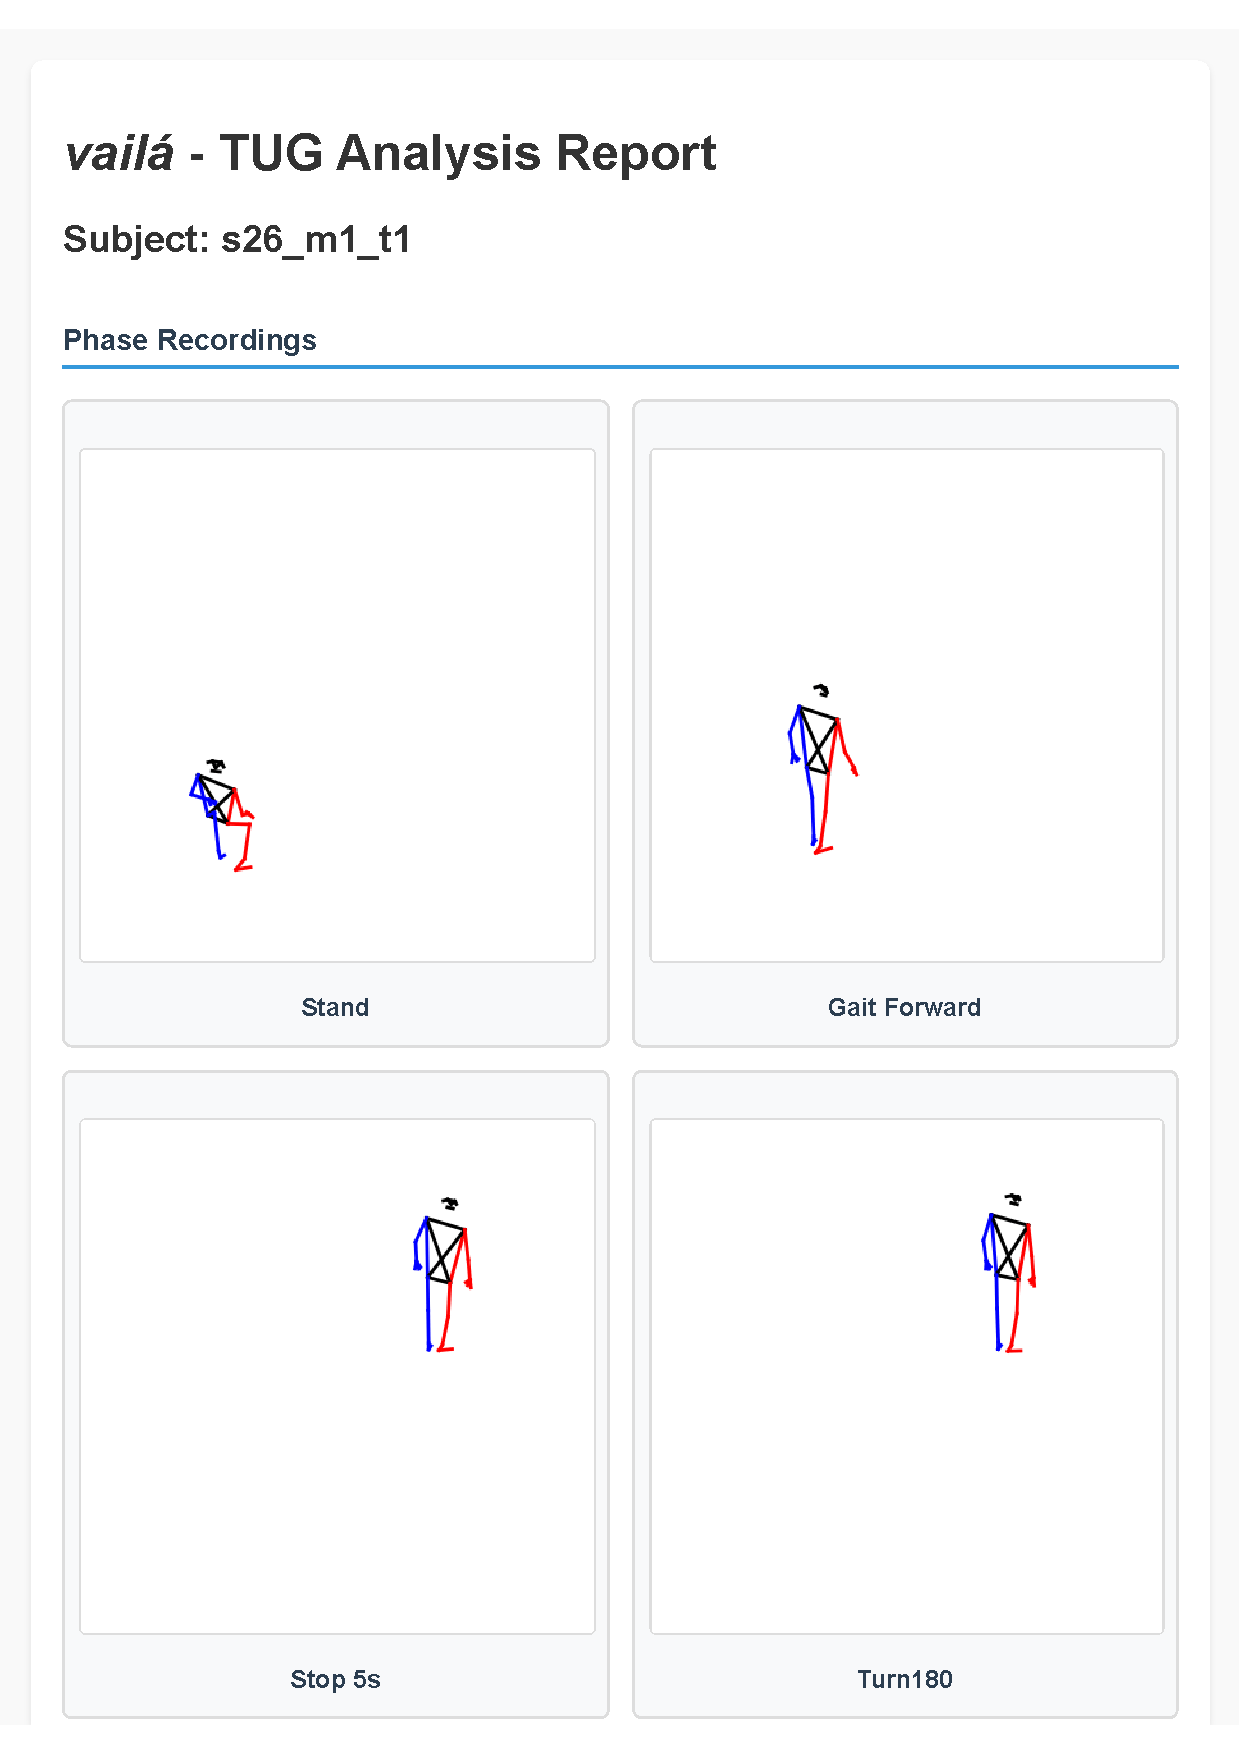
\includepdf[pages=-,pagecommand={}]{images/TUG Report_ s26_m1_t1.pdf}

\bibliographystyle{unsrtnat}
\bibliography{references}

\end{document}
